\documentclass{article}
\usepackage[margin=1in]{geometry}
\usepackage[shortlabels]{enumitem}
\usepackage[T1]{fontenc}
\usepackage[utf8]{inputenc}

\usepackage{graphicx,float}
\usepackage{amsmath,amssymb,amsthm,commath,xfrac}
\usepackage{hyperref}
\usepackage{cleveref,outlines}
\usepackage{booktabs,multicol}
\usepackage{lmodern,microtype,soul,siunitx}

\usepackage{todonotes}
\newcommand\todoin[2][]{\todo[inline, caption={2do}, #1]{ %inline todo box
  \begin{minipage}{\textwidth-4pt}#2\end{minipage}}}

\title{Room Draw Milestone 3}
\author{Daniel Metz, Eric Campbell, Kevin Wynn}
\date{December 16th, 2015}

\begin{document}
\maketitle

\section{Motivation}
\subsection{Ambitions}

We wish to implement an online transaction processing system for Pomona College
room draw. Our implementation is inspired by the current course registration
system.

\subsection{Functionalities}

Our ideal is a proof of concept of a working Room Draw replacement system. Our
core functionality includes:

\begin{outline}
\1 students signing up for singles, doubles, or friendship suites
\1 students to create draw groups
    \2 groups have a representative who controls group preferences
\1 students to search for rooms
    \2 offer filtering by property (e.g. taken, vacant, location, dorm, sq-ft,
    etc.)
\1 an ``auto draw'' system
    \2 We define an ``auto draw'' system as one in which students may provide an
    ordered list of room preferences, to allow for automated room selection at
    draw time given room availabilities.
\1 including all the actual rooms around campus
\end{outline}

Possible extensions include:

\begin{outline}
\1 include access to room reviews in system
\1 include a notification system
\1 include historical data as context for each room (another property of the
    room)
\1 permit 5C campus exchanges (e.g. CMC student living at Pomona)
\1 generation of room draw numbers/times
\1 administrator override (e.g. allow Bedoya to move students around or modify
    draw numbers/times).
\end{outline}

% \section{Group Organization}
% \subsection{Tasks, Roles, and a Timeline}
Daniel Metz will be the group member responsible for all submissions. He will
provide a publicly accessible GitHub repo at the termination of the project
containing all relevant code and documentation.

Furthermore, we foresee the following major tasks and assign members for each as
follows:

\subsection{Timeline}

\begin{table}[H] \centering
\begin{tabular}{ll} \toprule
Date & Task \\ \midrule
09/23 & milestone 1 (all) \\ \midrule
09/26 & ER diagram (Kevin) \\
09/26 & schema (Eric) \\
09/28 & business logic (Eric) \\
09/28 & web design (Daniel) \\ \midrule
10/07 & milestone 2 and presentation (all) \\ \midrule
10/18 & database tables implemented (Eric) \\
10/25 & Rails application models implemented (Eric) \\
10/28 & aggregate room data (all) \\
10/31 & generate students, groups, preferences, numbers (Daniel) \\
11/07 & website skeleton (Kevin) \\
11/15 & search (Kevin) \\
11/18 & group making (Daniel) \\
12/02 & preferences (all) \\
12/02 & application interface logic implemented (Eric) \\
12/02 & minimum viable project complete (feature freeze) \\
12/15 & documentation (all) \\
12/15 & presentation (all) \\ \midrule
12/16 & milestone 3 (all) \\
\bottomrule
\end{tabular}
\caption{Timeline and Deliverable}
\end{table}

\section{A High-Level Walkthrough}
  In this section, we detail a high-level backend design as well as the usage
  for generic users and adminstrators.

  \subsection{ER Diagram}
  We model our ER diagram (\Cref{fig:er-diagram}) after Pomona College's current
room draw system with a few modifications. Students may be members of various
draw groups, each of which must contain at least one student.

Furthermore, each \emph{Draw Group} must have a \emph{Representative} who will
select a \emph{Collection} of one or more \emph{Room}s for the group. The
collection's total capacity must match the size of the draw group.

Similar to the student/draw group coupling, a \emph{Room} is required to be a
part of exactly one collection. These collections represent individual rooms by
themselves and multiple associated rooms like two-room doubles and friendship
suites. A representative may \emph{Request} a collection and rank the request
for automated room draw; this set of requests and rankings makes up the group's
preferences list. The priority of a request is determined by
\emph{rank\_absolute} which is a function of a draw group's \emph{draw\_num} and
the importance of that request for a draw group relative to their other
requests.

The \emph{Occupy} relation will be set by our AutoDraw system, assigning a draw
group to a collection in accordance with the totally ordered set of all
requests. This allows students in a draw group to later assign themselves to
appropriate rooms within an assigned collection in accordance with the joint
decisions of the members of the draw group.

\begin{figure}[H] \centering
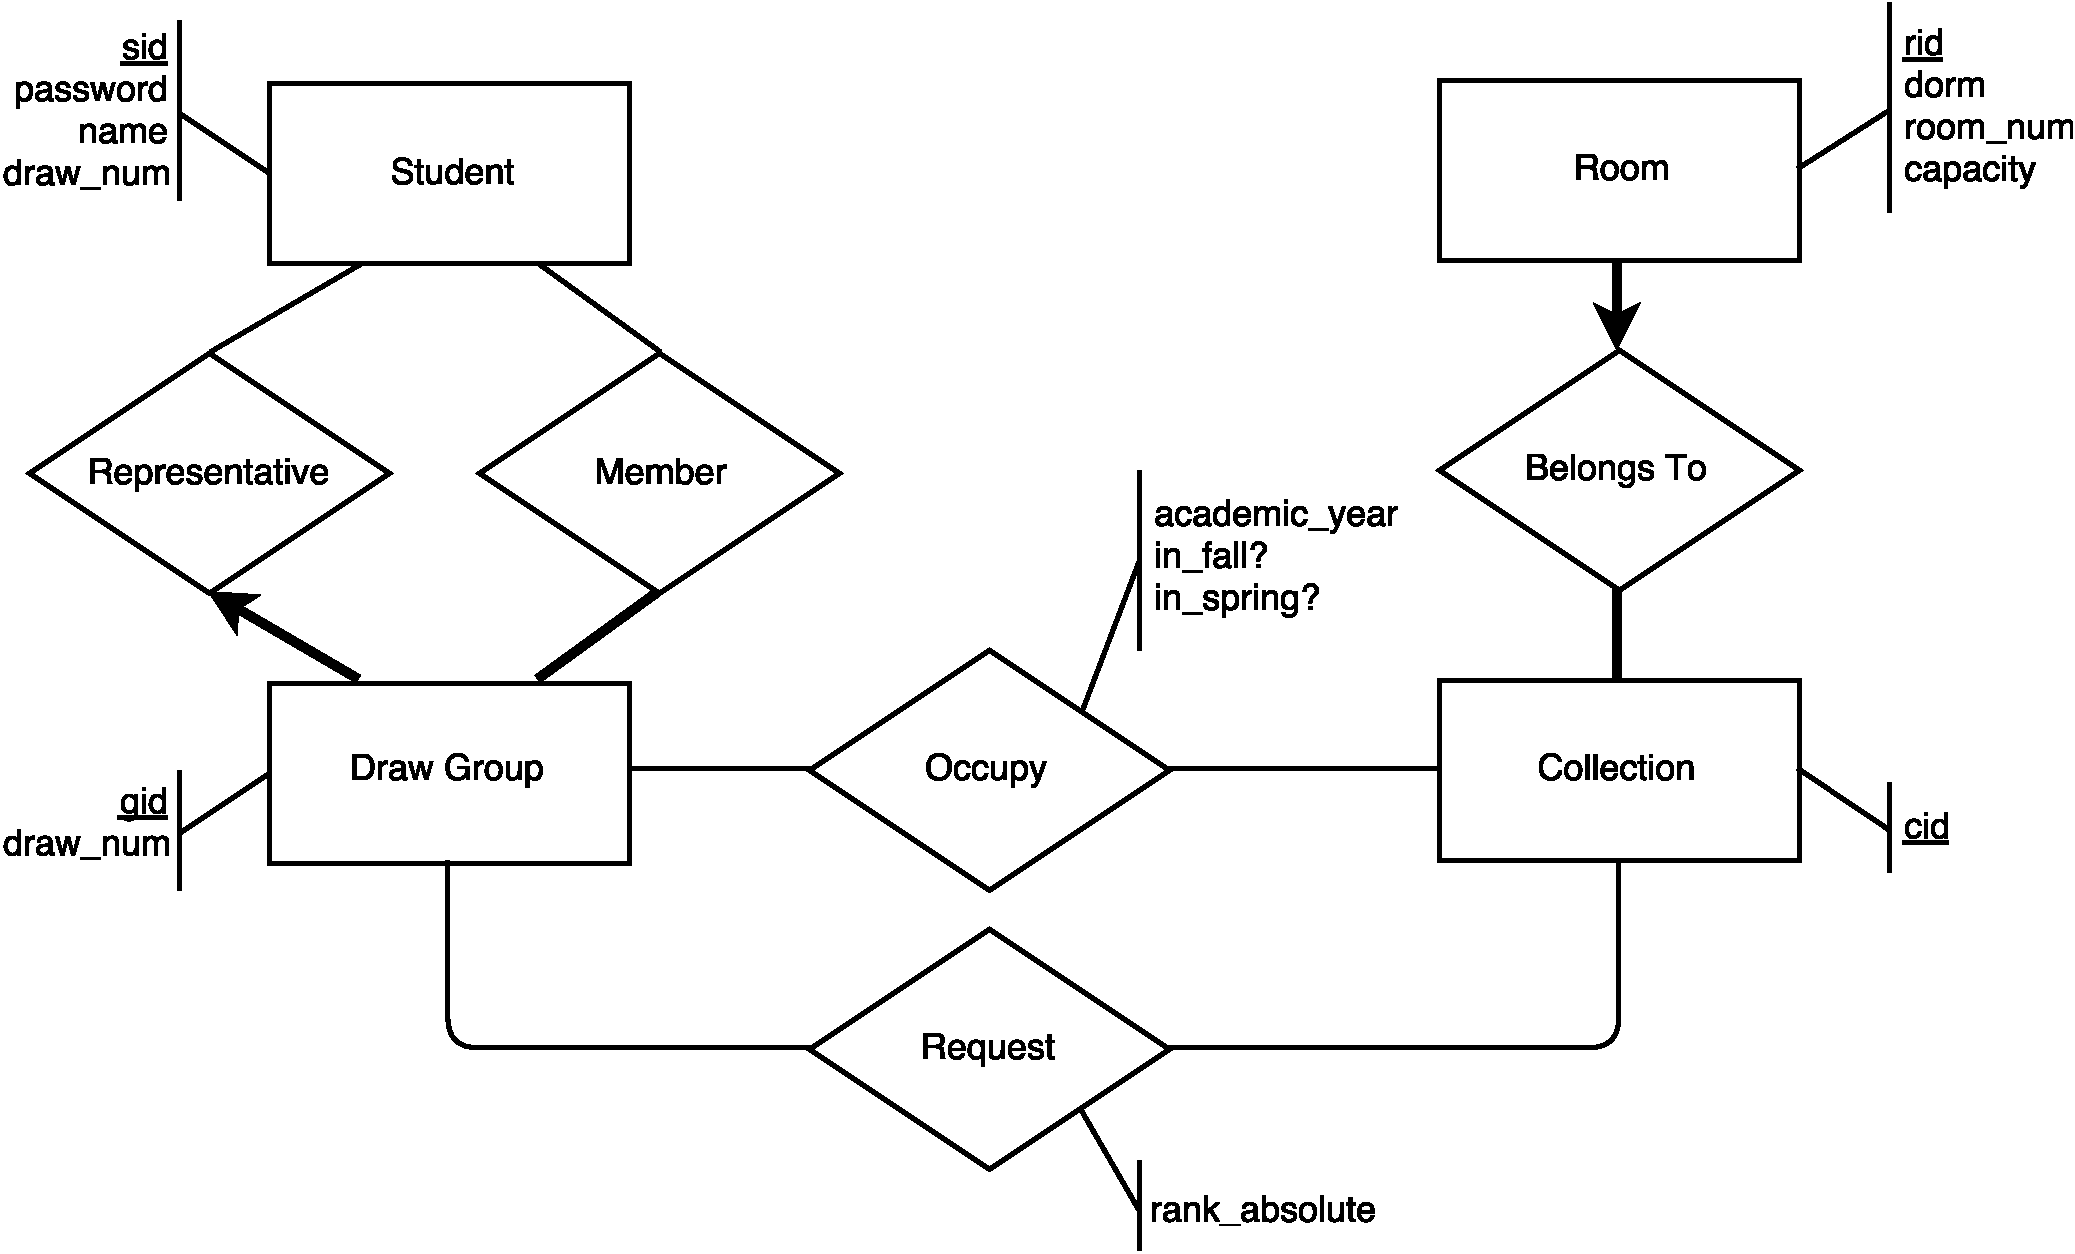
\includegraphics[width=\textwidth]{er_crop.pdf}
\caption{Our ER Diagram}
\label{fig:er-diagram}
\end{figure}


  \subsection{User Manual}
  \begin{outline}
\1 Login Page

  \2 The login-page prompts a user to log-in with a student id and password.
  Currently the set of user ids and passwords are independent of those used by
  Pomona College. Note however the system does consider security, and stores
  only password digests encrypted via \texttt{bcrypt}.
  \2 Before Room Draw:
    \3 Upon successful log-in, a student is notified that they do not yet have
    an assigned room. They are also provided with simple navigational
    instructions.
  \2 After Room Draw:
    \3 If a student belongs to a draw group that has successfully drawn into a
    collection, the student is brought to a landing page informing the student
    of such. This lists the students with whom they will be living, and the
    rooms that are collectively assigned. GUI access to other features of the
    site is disabled.
    \3 Otherwise, if none of a student's draw groups have been successfully
    assigned to a collection, the web-app behaves as if AutoDraw has not yet
    been run.

\begin{figure}[H] \centering
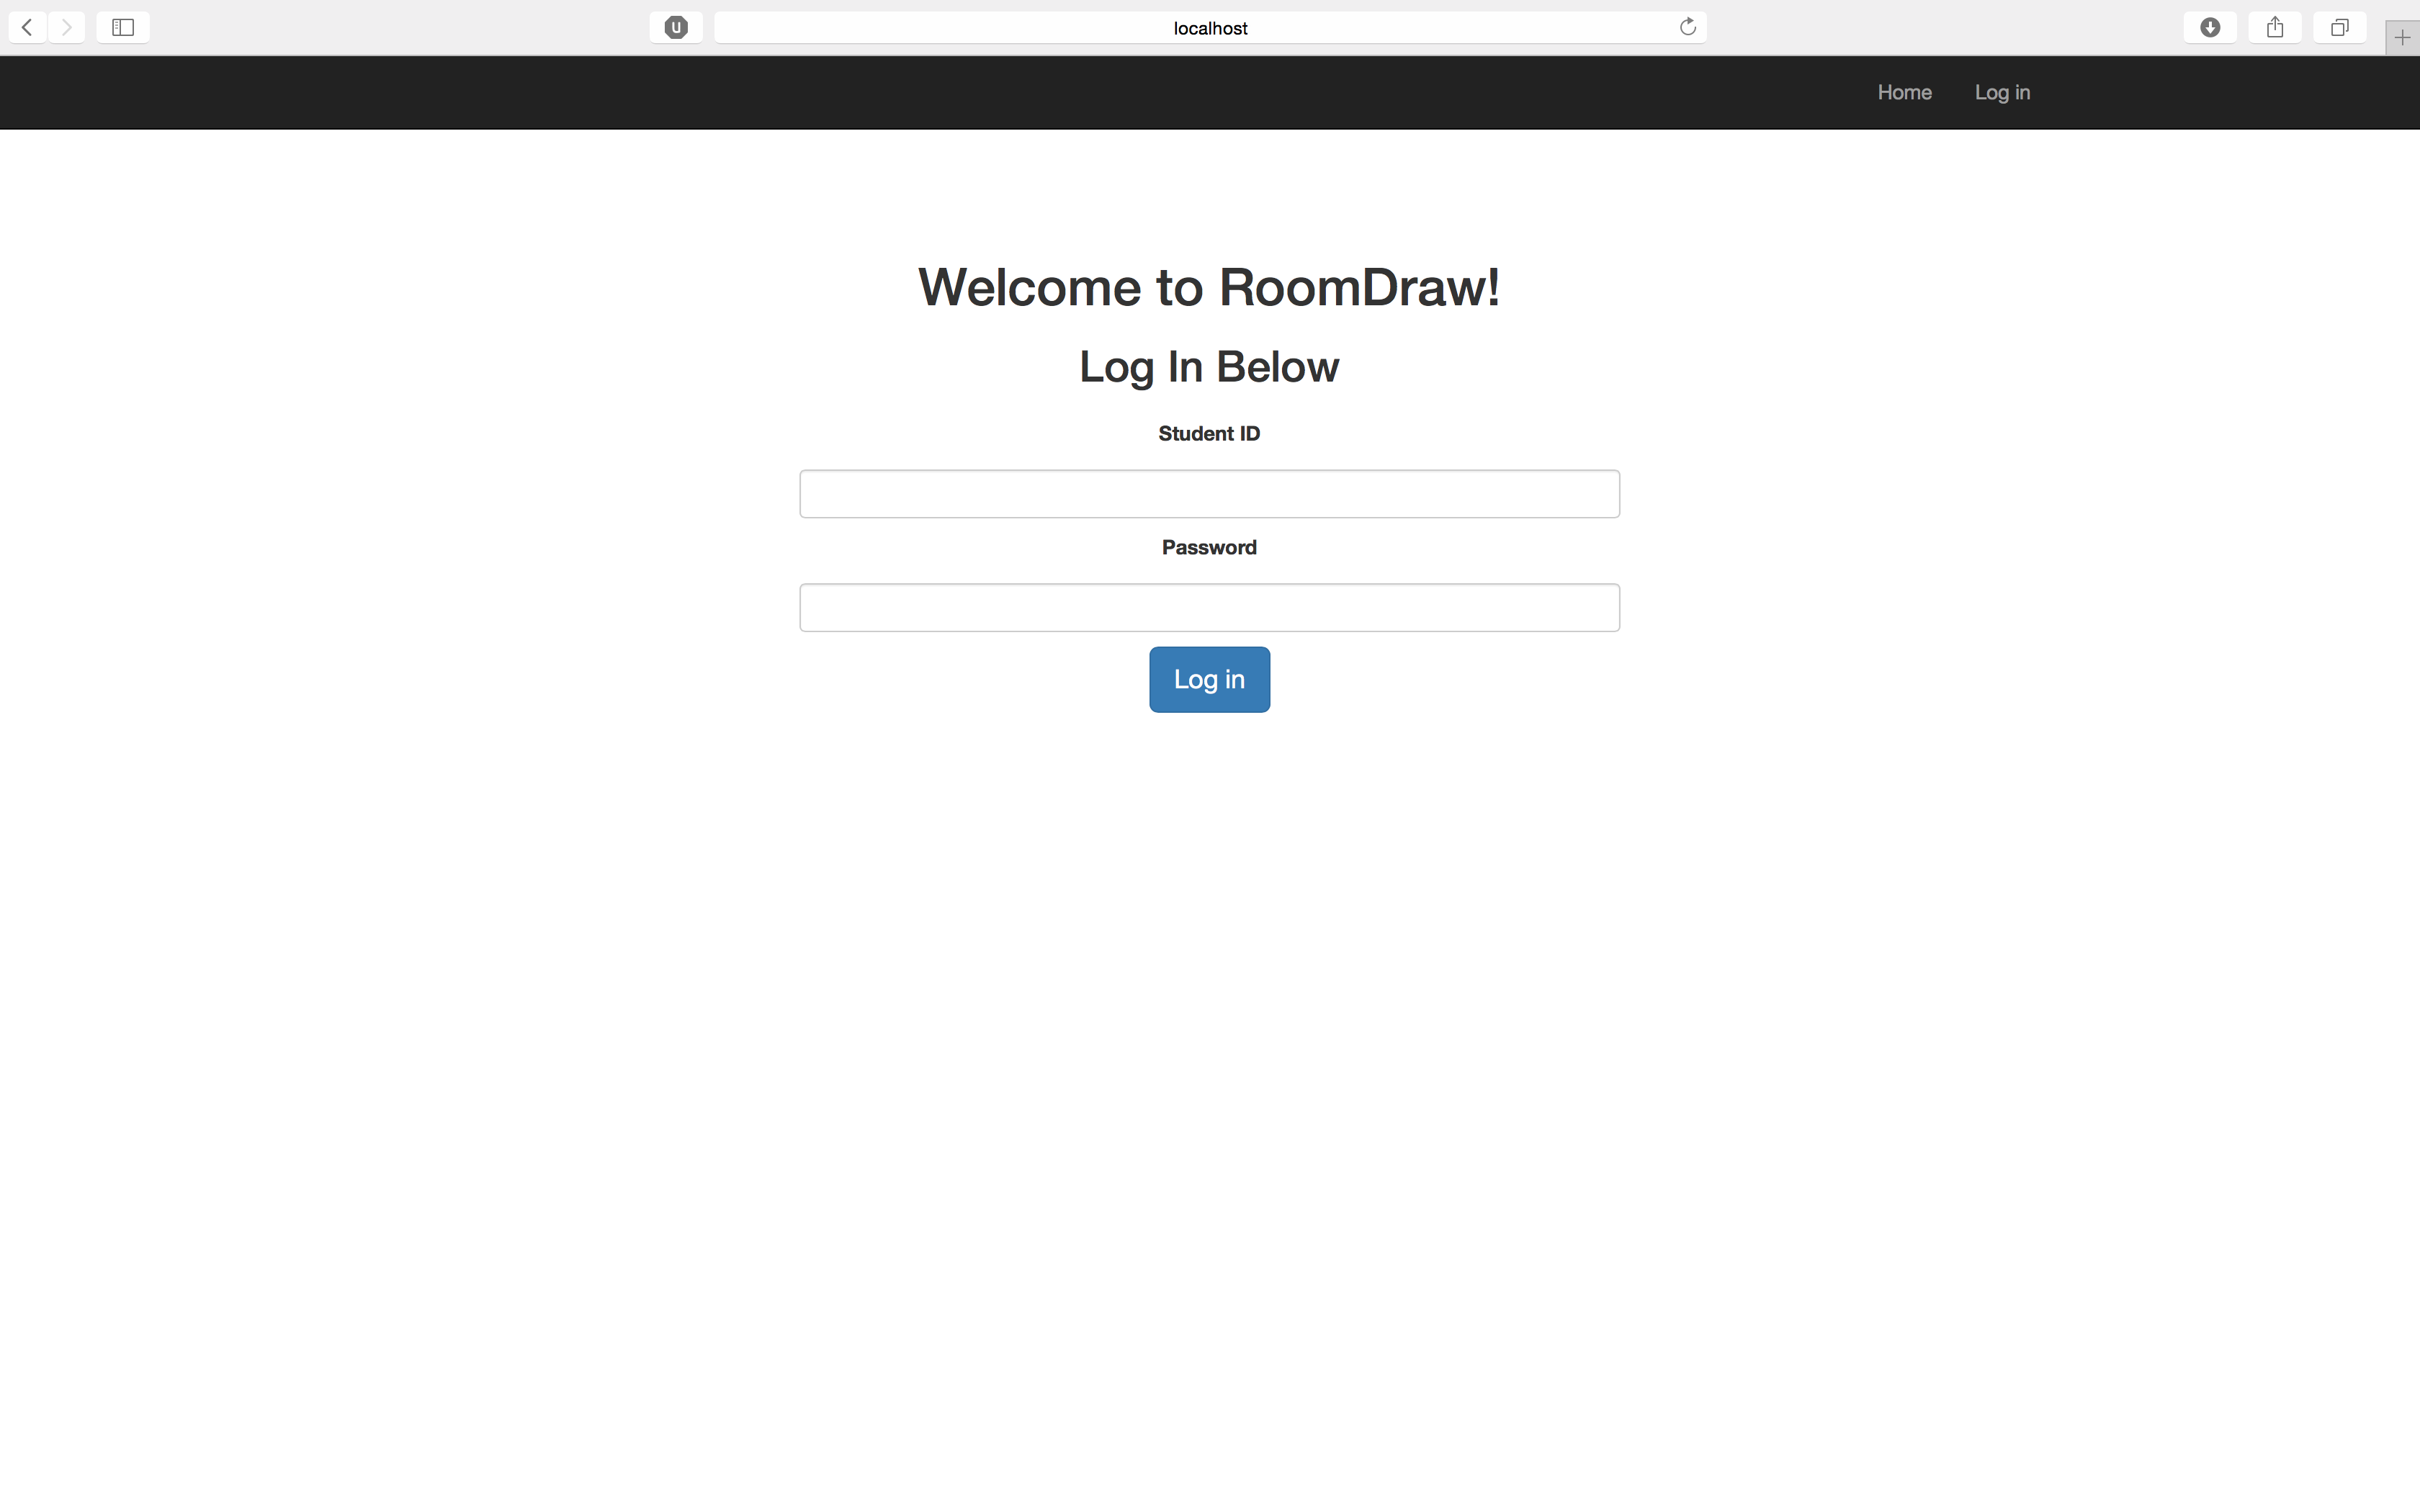
\includegraphics[scale=.225]{screens/login}
\caption{The Login Page}
\label{fig:screenlogin}
\end{figure}

\begin{figure}[H] \centering
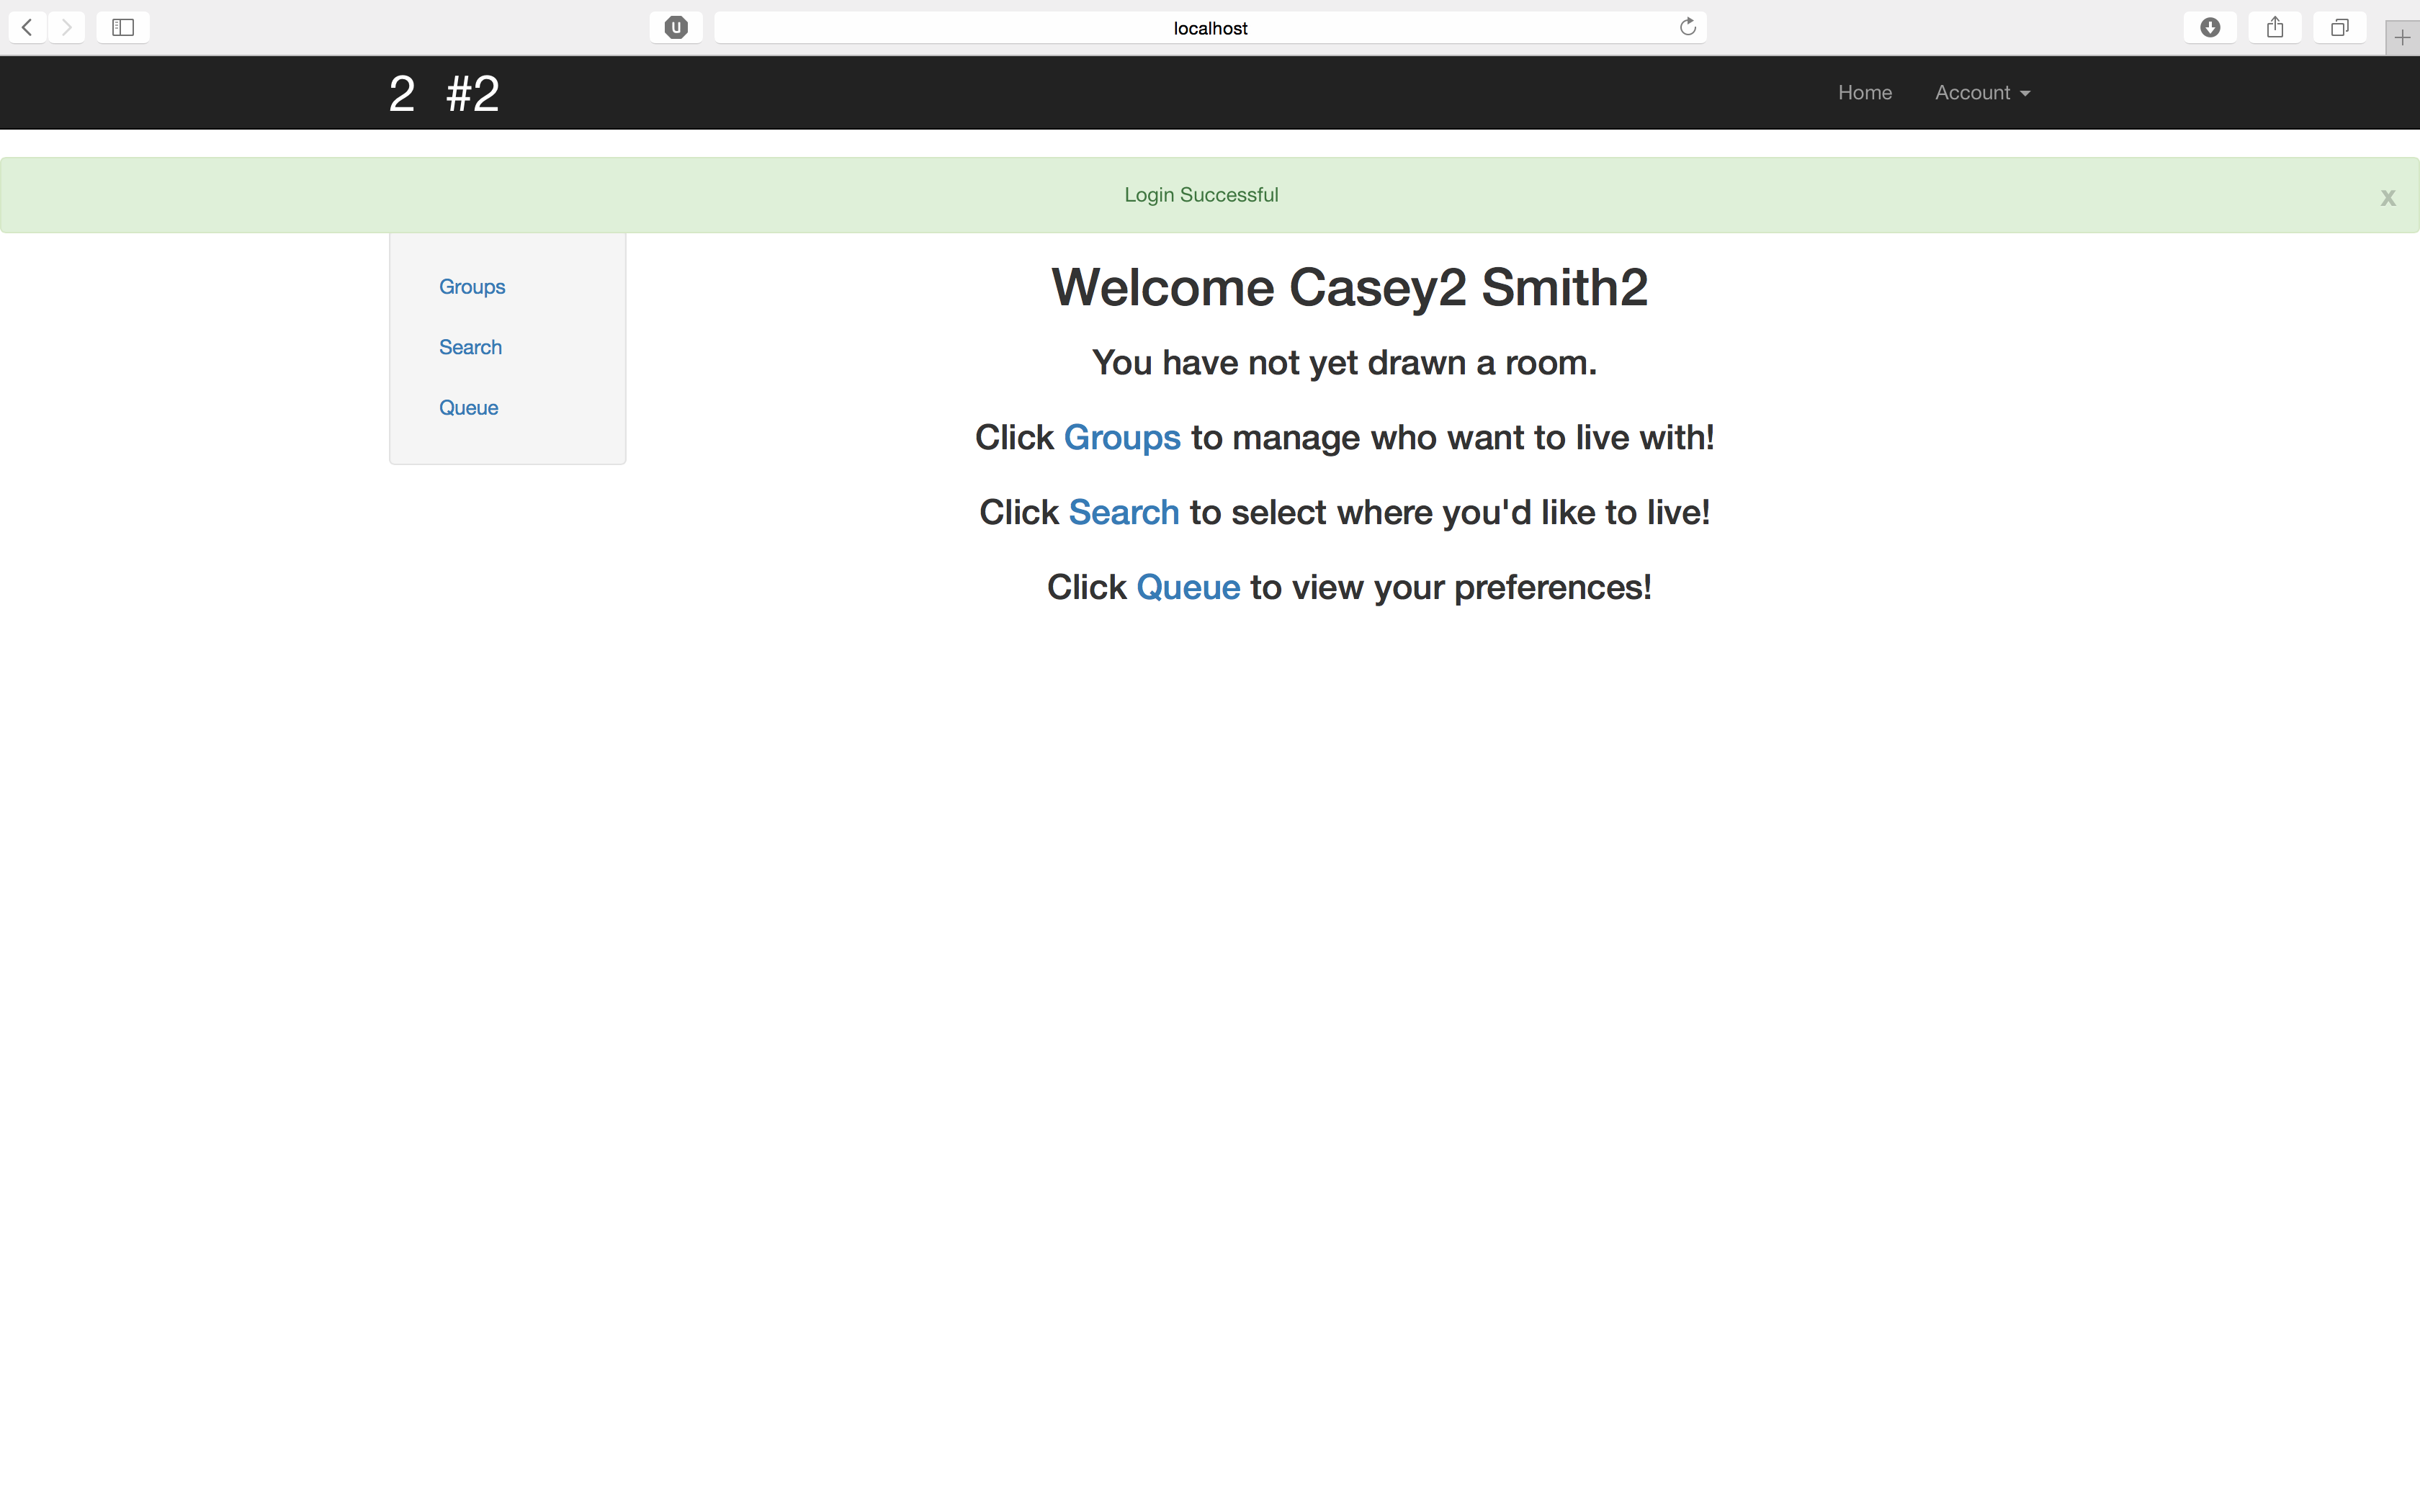
\includegraphics[scale=.225]{screens/landing_undrawn}
\caption{The Landing Page, Before Room Draw}
\label{fig:screenlandingundrawn}
\end{figure}

\begin{figure}[H] \centering
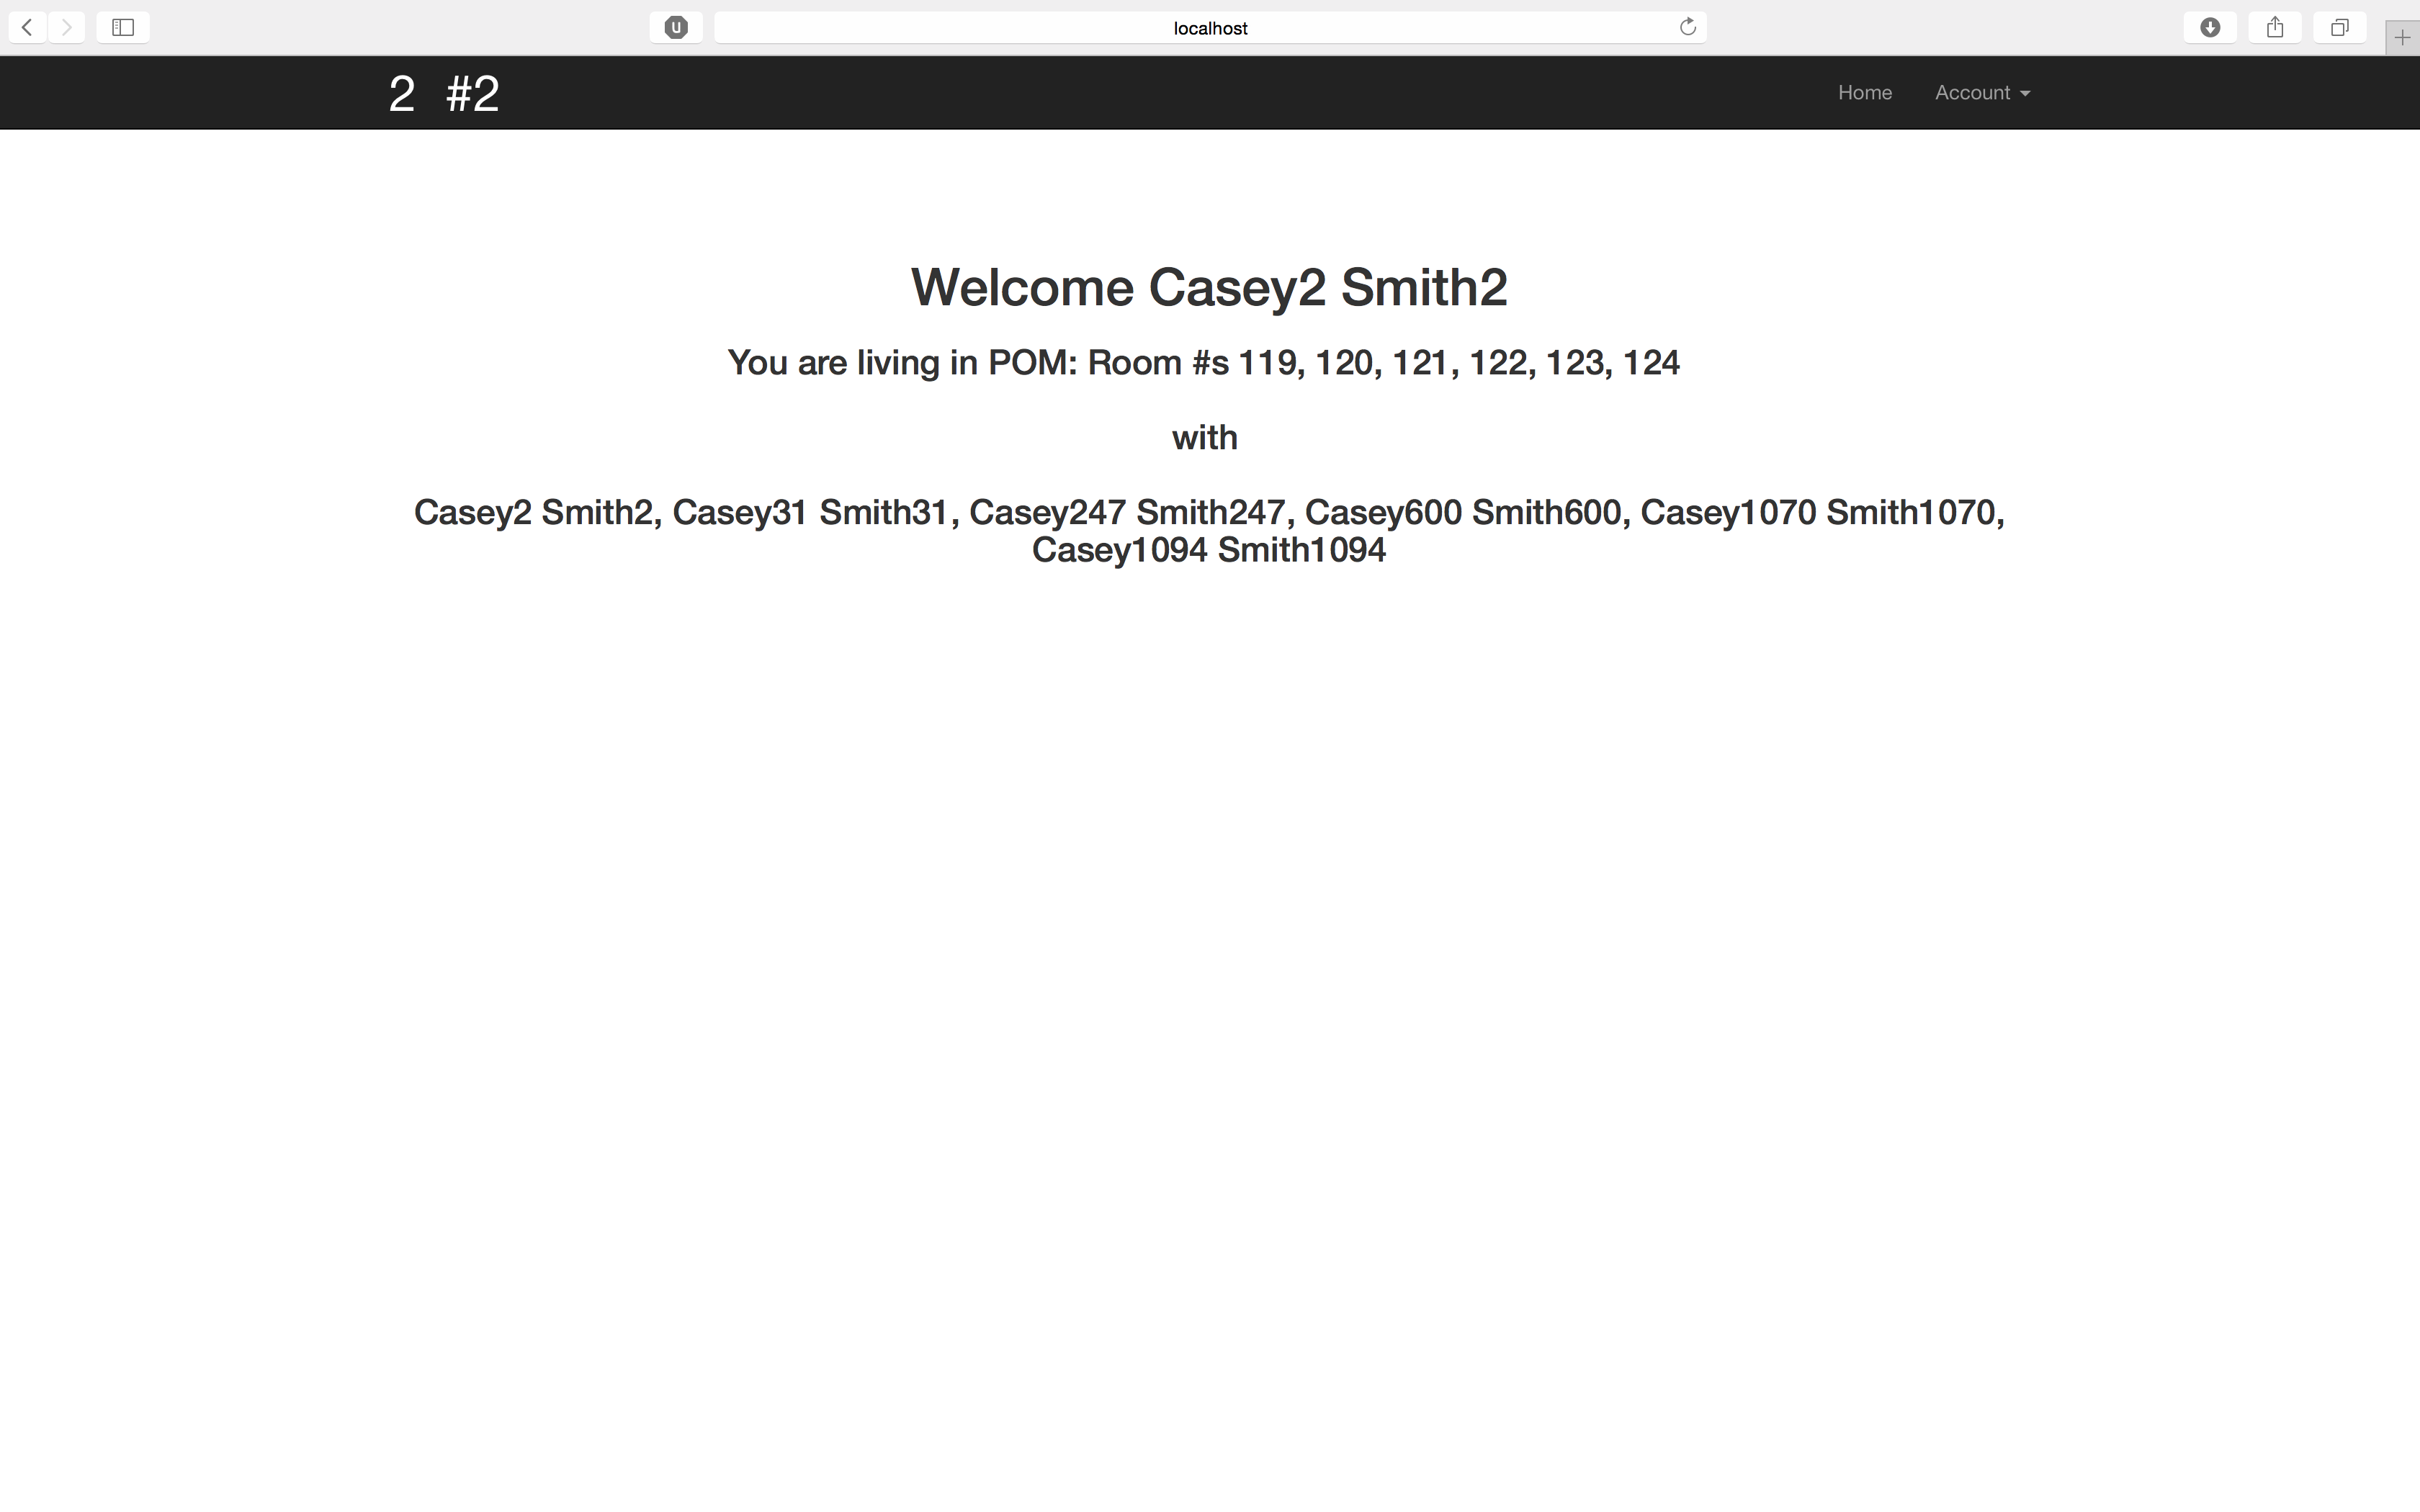
\includegraphics[scale=.225]{screens/landing_drawn}
\caption{The Landing Page, After Room Draw}
\label{fig:screenlandingdrawn}
\end{figure}

\1 Group Management

  \2 By default, all students belong to a group containing only themselves.
  \2 All students may create additional draw groups (up to a max of 50). Doing
  so will create a new draw group, initialized to contain the logged-in student.
  \2 Any student belonging to a draw group may add any other student to that
  group via student id. Draw groups are capped at size 6. Draw groups containing
  between 3 and 6 members are considered friendship groups, and have their draw
  numbers calculated by average.
  \2 Any student belonging to a group may delete it, which removes all data
  associated with that group.

\begin{figure}[H] \centering
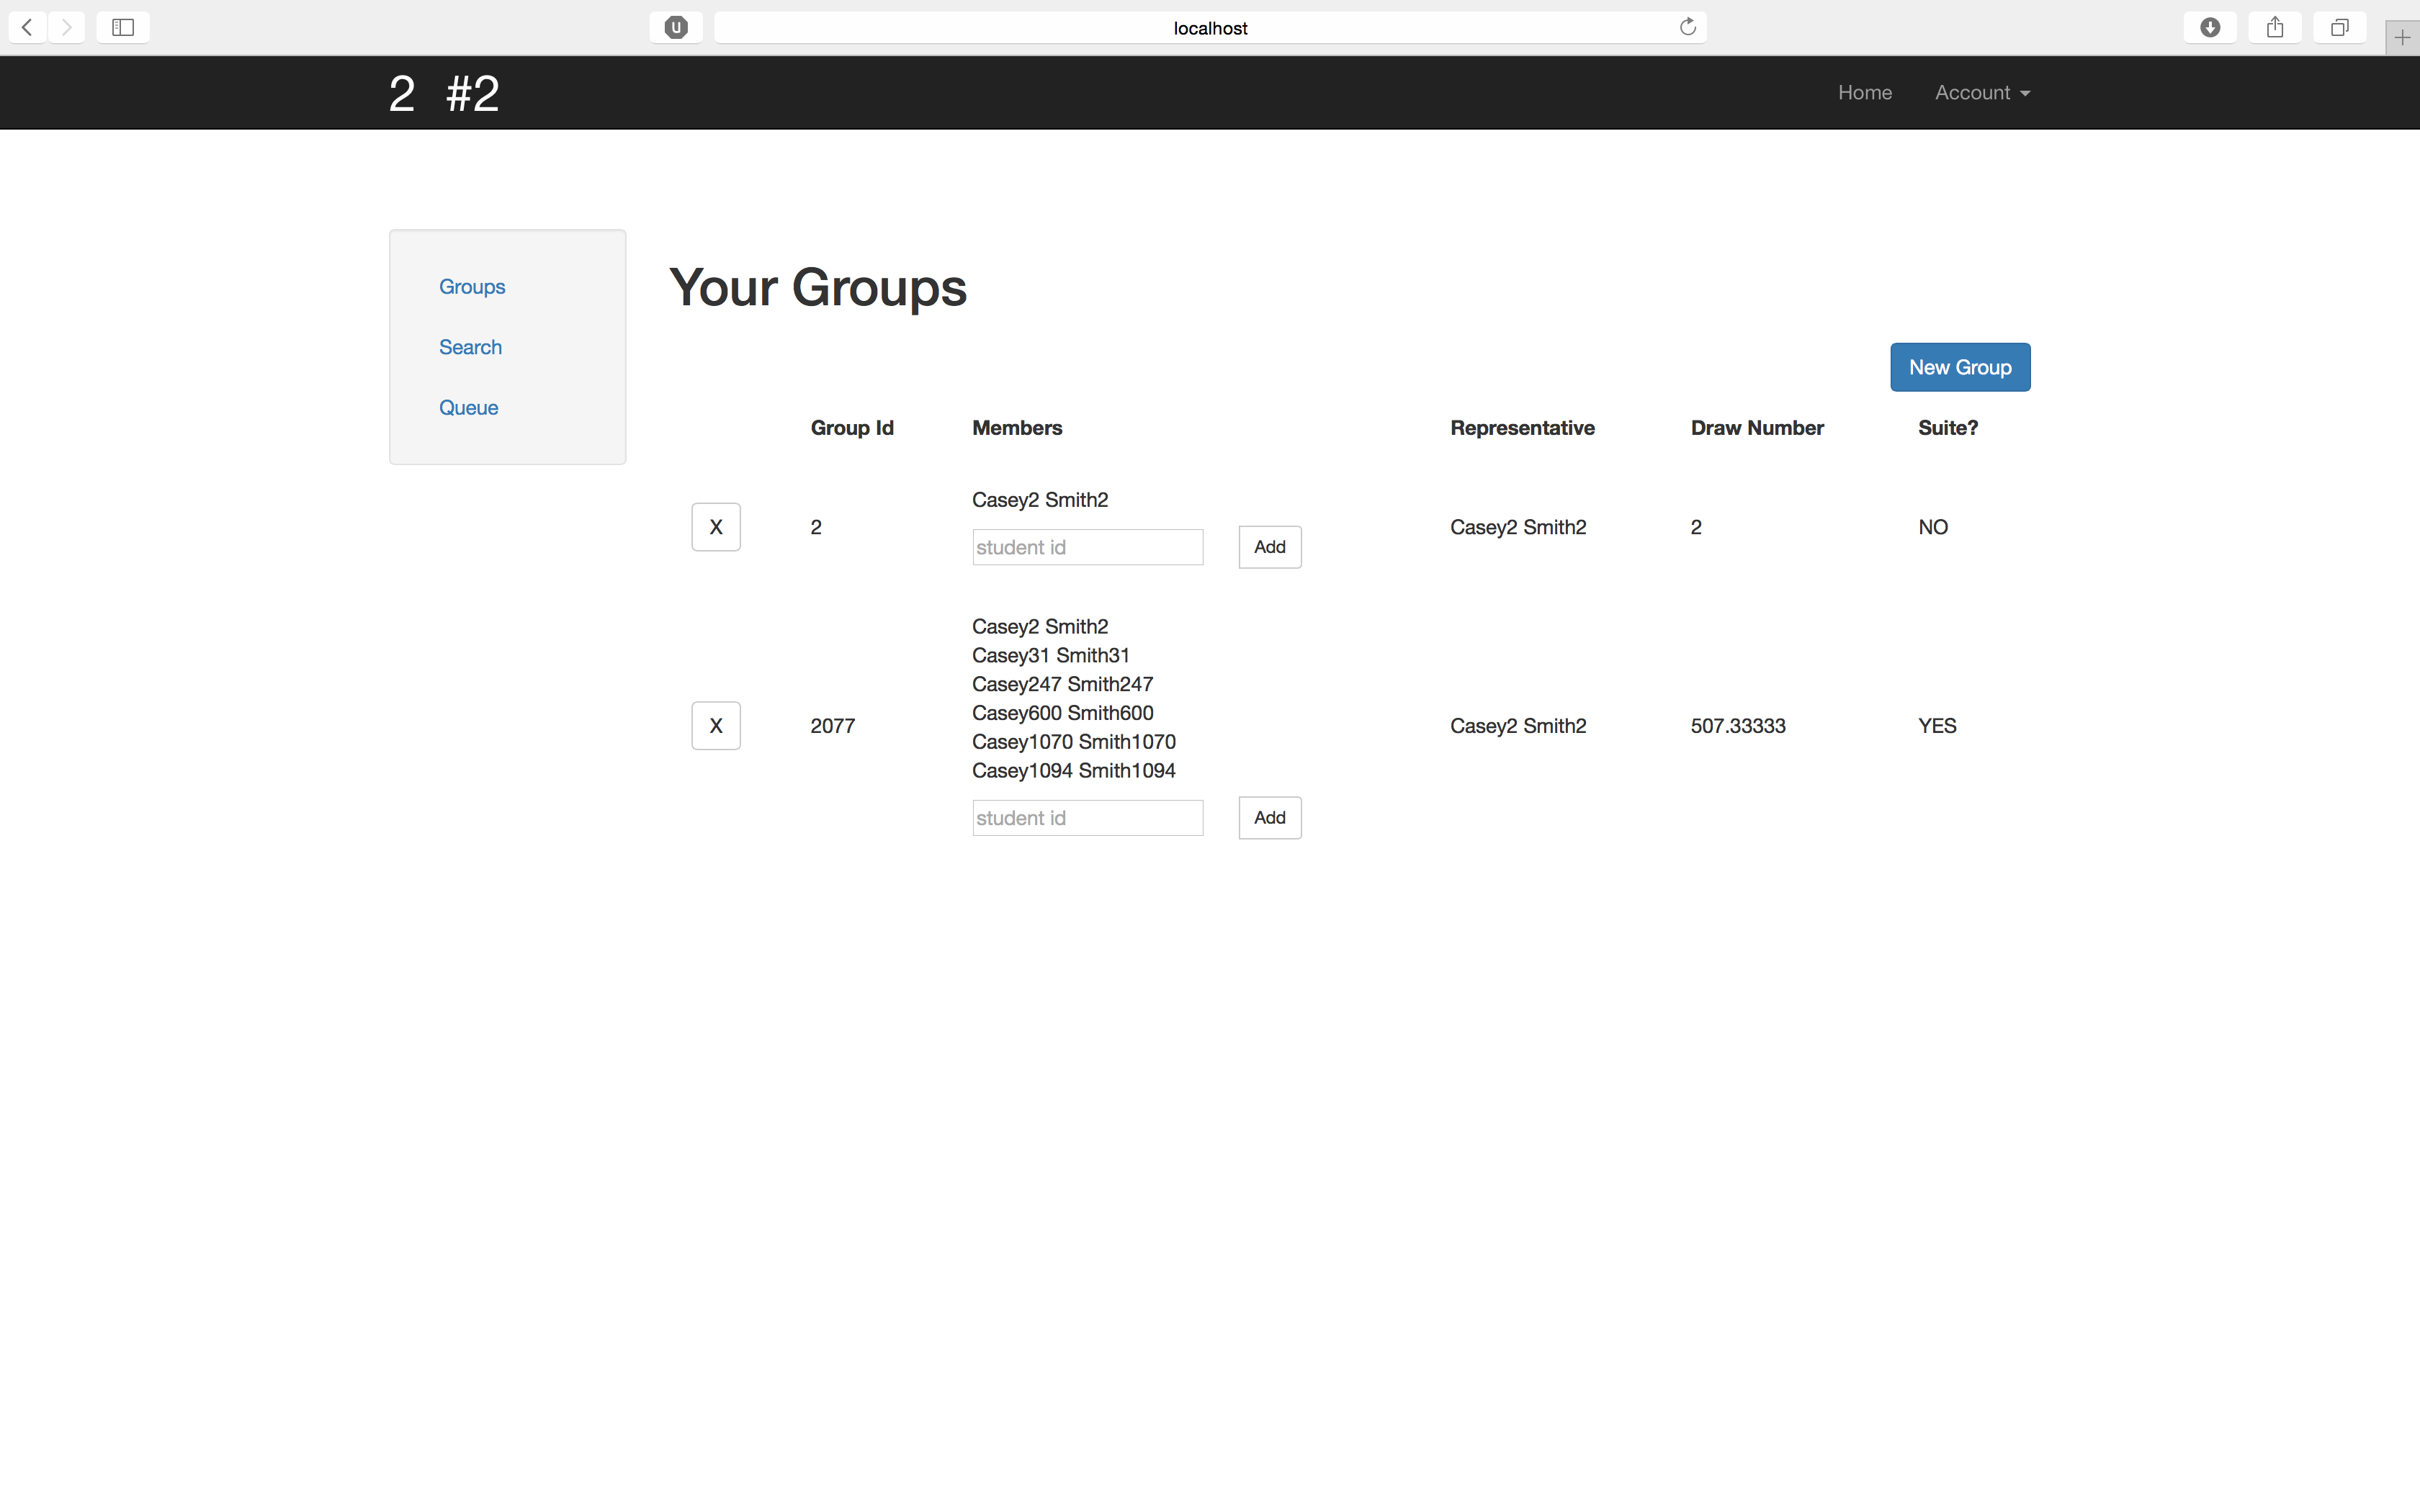
\includegraphics[scale=.225]{screens/group}
\caption{The Group Management Page}
\label{fig:screengroup}
\end{figure}

\1 Collection Search

  \2 The search page supports search by dorm name and by collection capacity.
  For each matching collection, the collection id, dorm name, room number(s),
  and room capacity(-ies) are listed. Group representatives may select a group
  they represent and add the collection to that group's preferences queue.

\begin{figure}[H] \centering
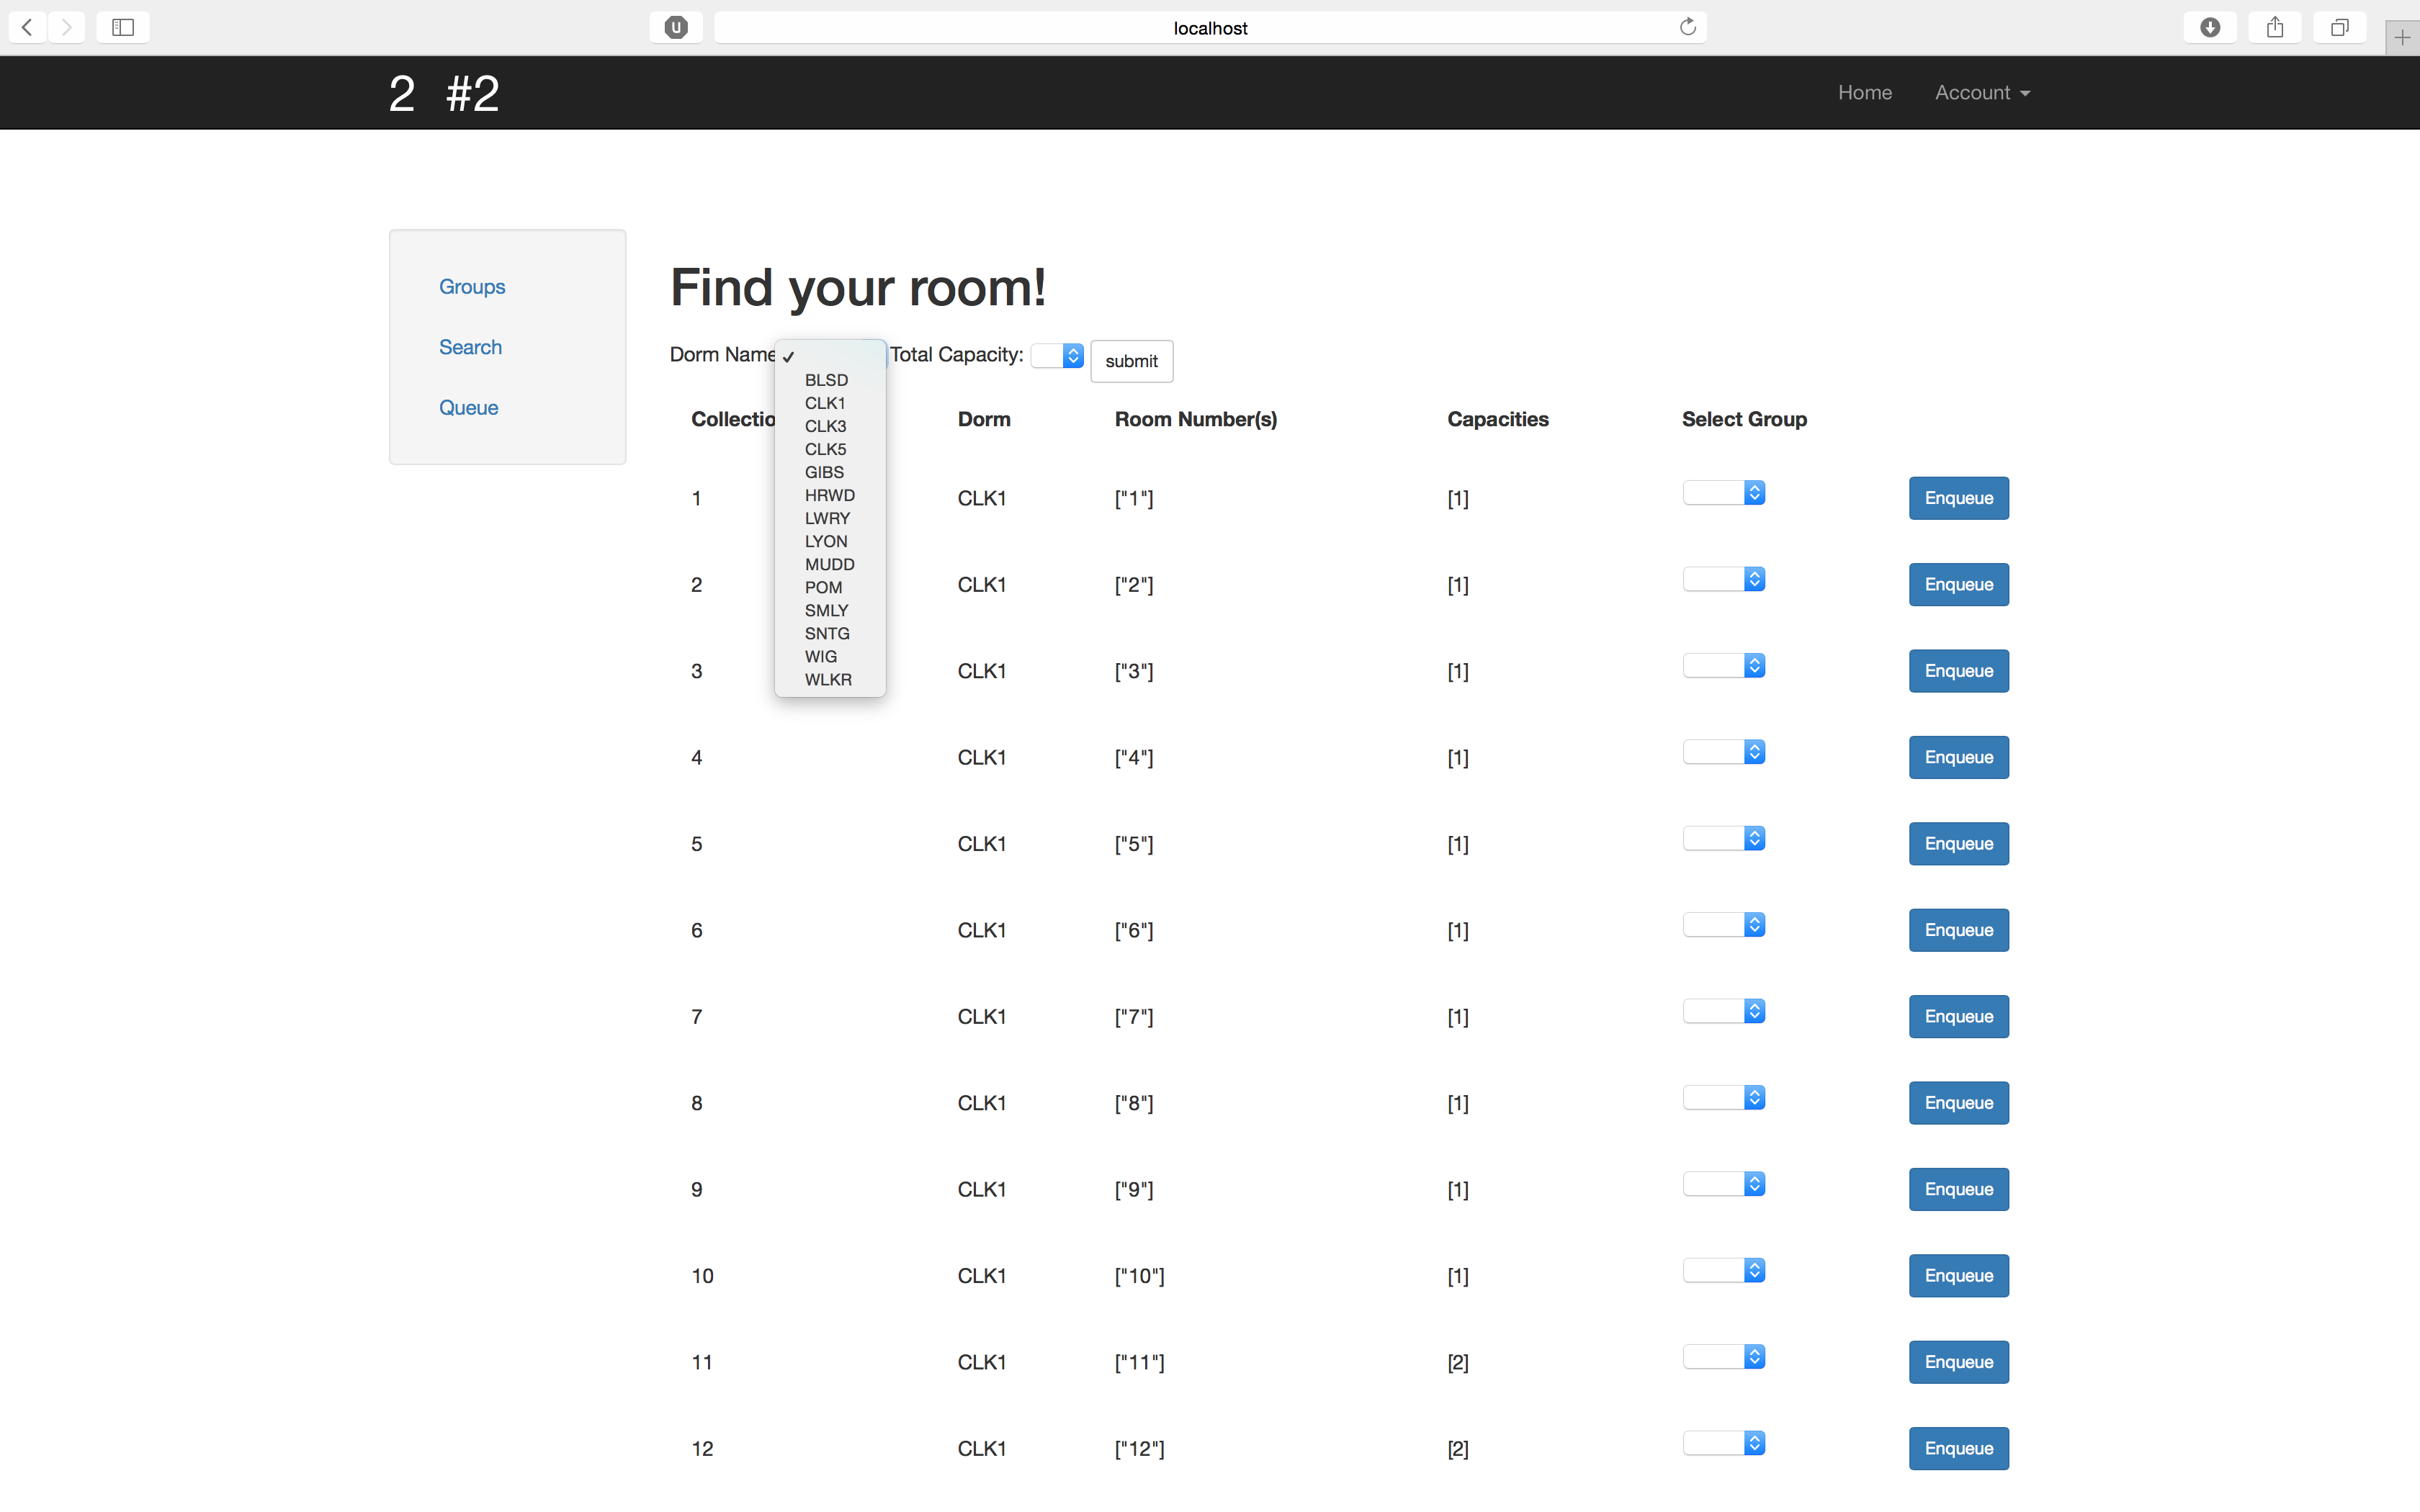
\includegraphics[scale=.225]{screens/search}
\caption{The Search Page}
\label{fig:screensearch}
\end{figure}

\1 Preference Queue

  \2 The Queue page lists out the various requests made by groups to which the
  logged-in student belongs. These requests are sorted first by the draw numbers
  of the groups, then by their addition time to the queue. We offer a small
  example to illustrate our intent: Consider that I add to my queue collection
  \(a\) for my solo group. I then add to my queue collection \(b\) for a
  friendship group I represent. I lastly add collection \(c\) for my solo group.
  The queue will display results in order \(b, a, c\), mirroring the order by
  which the requests would be evaluated at the moment of AutoDraw.
  \2 Requests in the queue may be deleted.

\begin{figure}[H] \centering
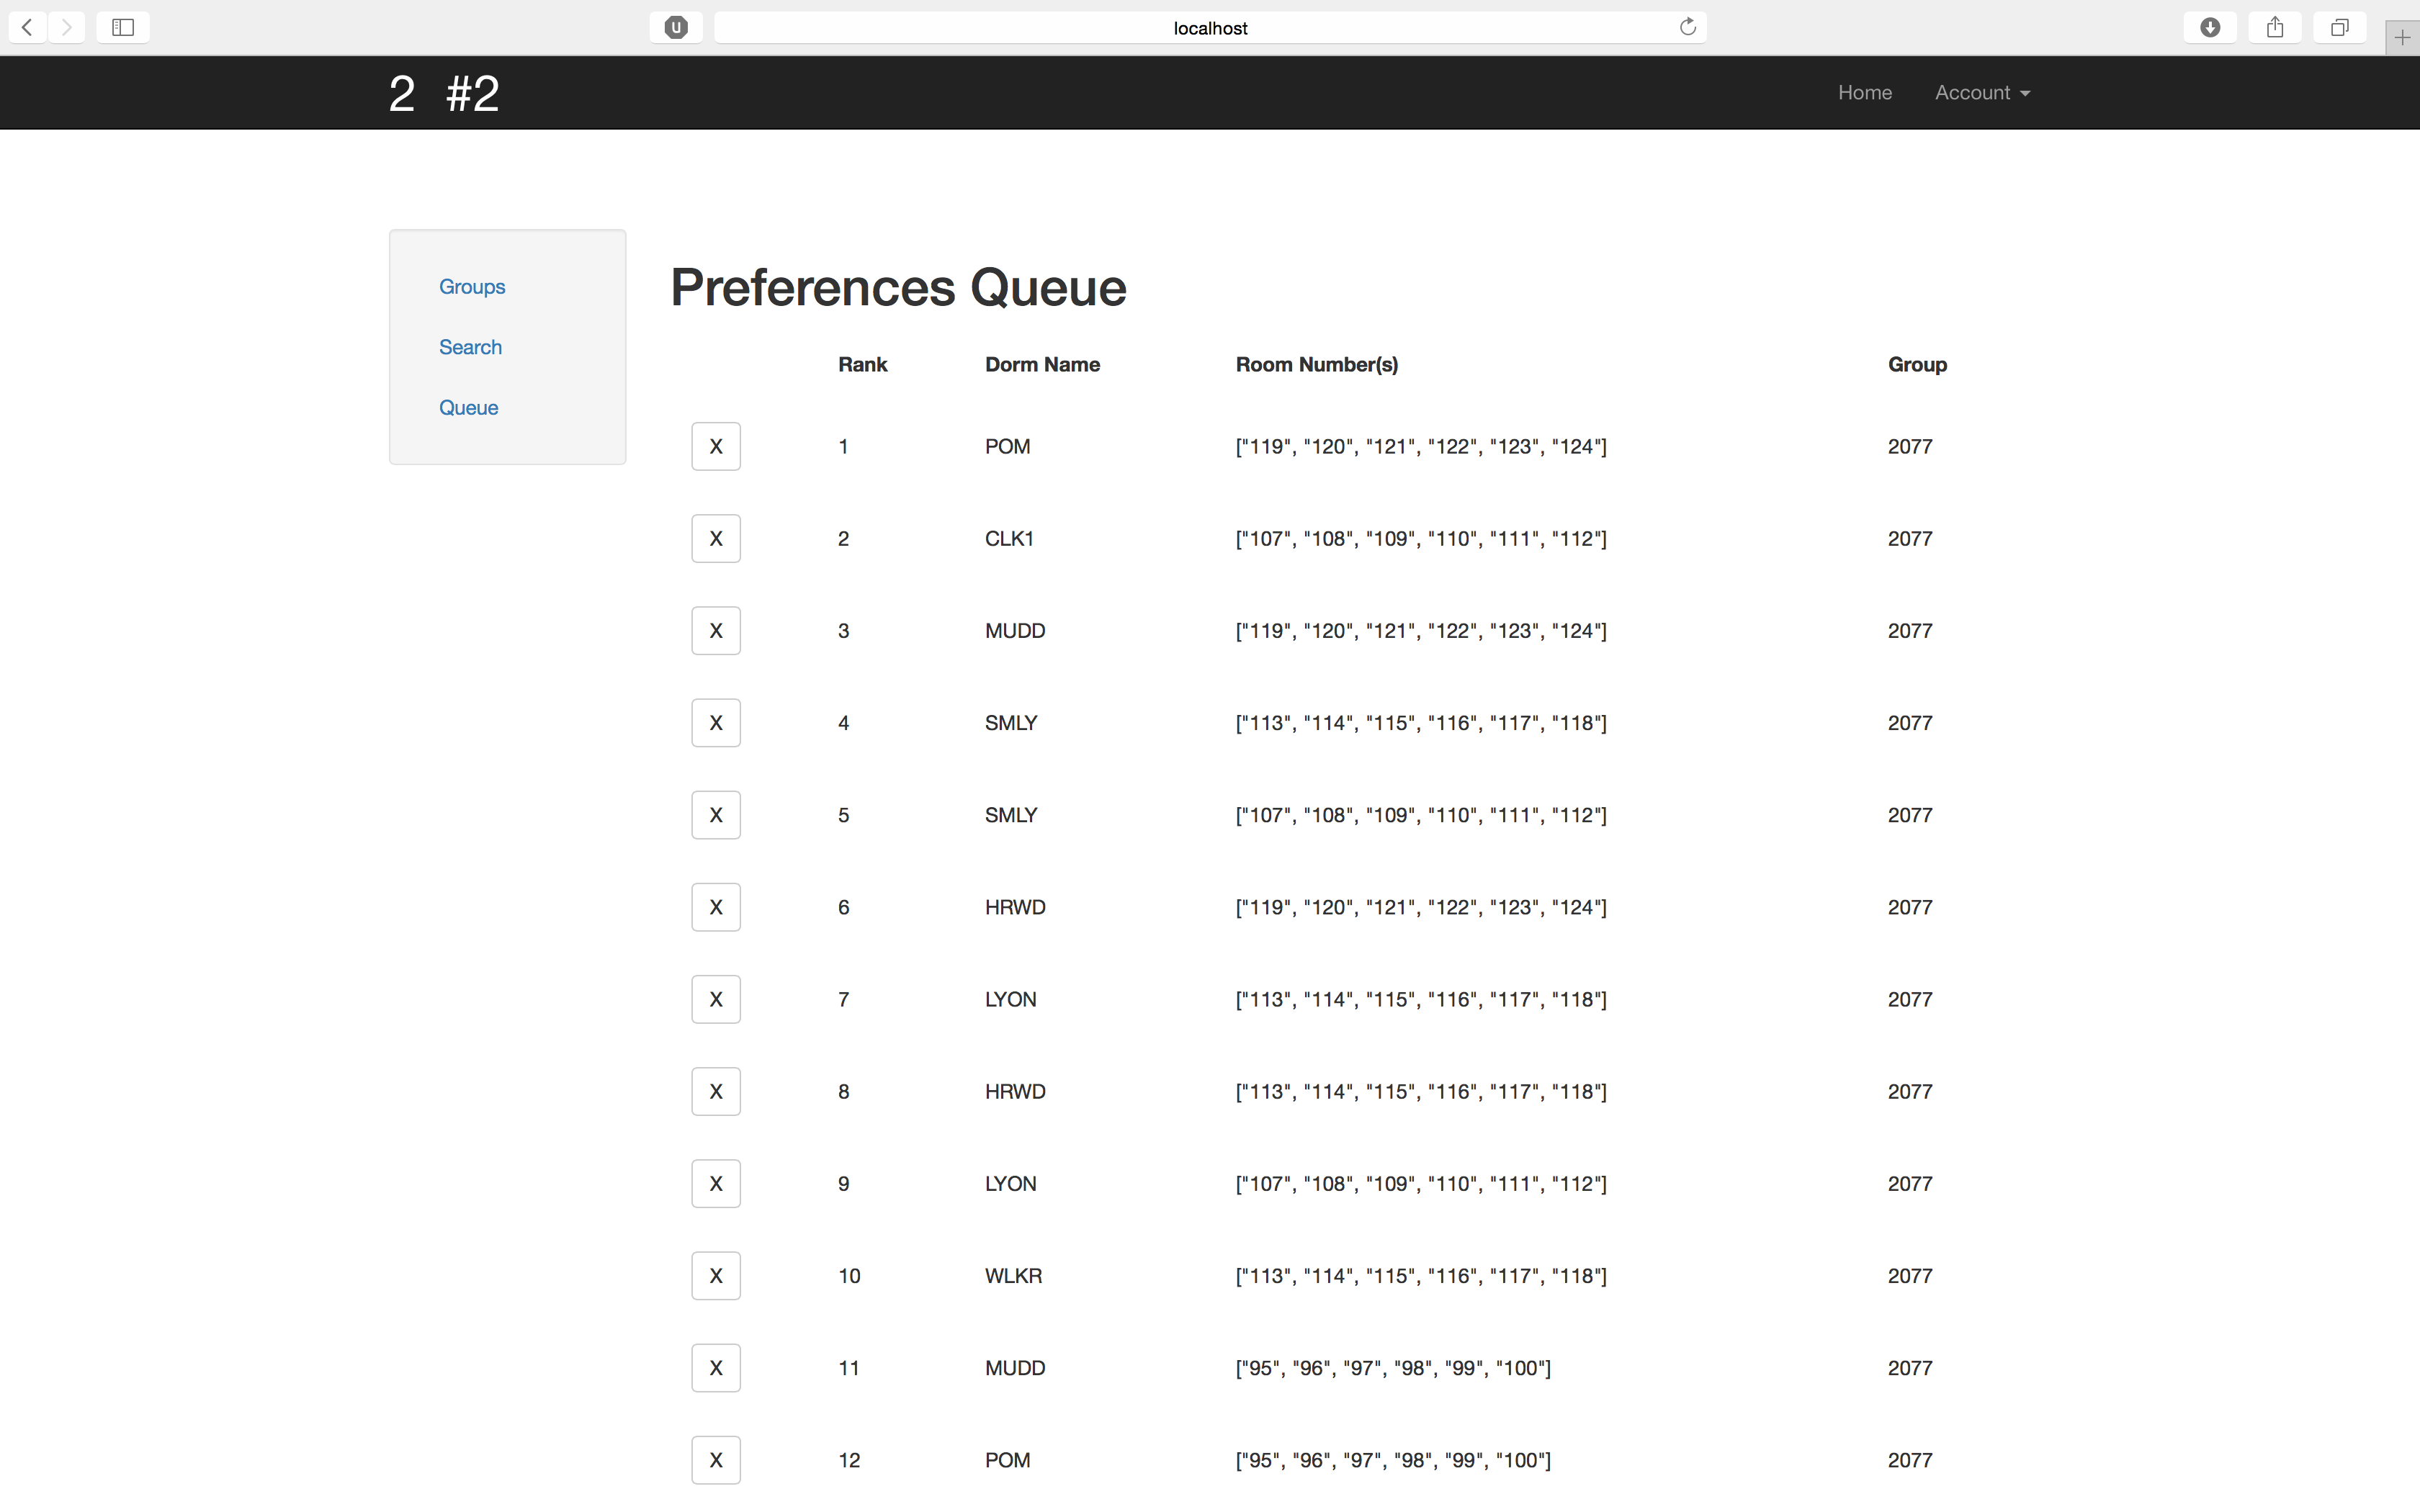
\includegraphics[scale=.225]{screens/queue}
\caption{The Preference Ranking Page (Queue)}
\label{fig:screenqueue}
\end{figure}

\end{outline}


  \subsection{Admin Manual}
  The automated room draw task (AutoDraw) assigns draw groups to collections in
order of absolute ranks. At the end of the task, it is possible that a user will
not have been drawn into a room. Such users must then update their preferences
and the task must be rerun for these individuals. This \texttt{rake} task must
be run on the production database, hosted by Heroku, by calling \texttt{heroku
run rake draw:auto[year]} where \texttt{year} is the fall academic year for
which users are drawing.

In order to perform the task, admin privileges on the Heroku app are required.
The admin should install Heroku toolbelt (\url{https://toolbelt.heroku.com}) and
navigate to a local repository of the project which can be found at
\url{http://github.com/danielmmetz/cs133_project}. Here, use the command
\texttt{heroku login} and follow the output instructions to finish set up. Once
this is completed, the aforementioned \texttt{rake} task may be run.

\section{Low Level Details}
  \subsection{Schema}
  The result of the translation of the ER diagram to the schema is presented in
the next section, as well as the explanation of any non-obvious choices. First,
consider the \emph{Student} and \emph{DrawGroup} entity sets and their mutual
relationships.

\begin{description}
  \item Student(
        \ul{\emph{student\_id}: \texttt{integer}},
        \emph{password}: \texttt{string},
        \emph{draw\_num}: \texttt{integer},
        \emph{name}: \texttt{string},
        \emph{grad\_year}: \texttt{integer})

  \item Member(
        \ul{\emph{student\_id}: \texttt{integer},
        \emph{draw\_group\_id}: \texttt{integer}})

  \item DrawGroup(
        \ul{\emph{draw\_group\_id}: \texttt{integer}},
        \emph{draw\_num}: \texttt{integer},
        \emph{student\_id}: \texttt{integer},
        \emph{for\_suite}: \texttt{boolean})
\end{description}

The above schema mostly sticks to the obvious translation.  However, we have key
and total participation constraints on the \emph{Representative} relationship
with \emph{DrawGroup}. Since every entity in \emph{DrawGroup} must participate
in the \emph{Representative} relationship exactly once, \emph{student\_id} is a
foreign key to the \emph{Student} table in each \emph{DrawGroup} tuple. The
above schema is in Third Normal Form. \\

Now, consider a parallel set of entity sets \emph{Room} and \emph{Collection}.

\begin{description}
  \item Room(
        \ul{\emph{dorm\_name}: \texttt{string},
        \emph{room\_num}: \texttt{string}},
        \emph{capacity}: \texttt{integer},
        \emph{collection\_id}: \texttt{integer})

  \item Collection(
        \ul{\emph{collection\_id}: \texttt{integer}},
        \emph{suite\_num}: \texttt{integer})
\end{description}

Here there are total participation and key constraints on \emph{Room} with
respect to the \emph{Belongs\_To} relationship.  Since each and every entity in
\emph{Room} is in \emph{Collection} exactly once, the \emph{collection\_id} can
be an attribute in \emph{Room}. It is a foreign key to the
\emph{Collection} table. Here, Third Normal Form is maintained.

Consider the tables representing the \emph{Request} and \emph{Occupy}
relationships. The former is a straightforward translation. However, the latter
is not as intuitive. We have key constraints on the attributes listed below to
ensure that a \emph{DrawGroup} can only occupy at most a single collection per
semester in an academic year. We have also implemented business logic checks to
manage the different condition combination cases.

\begin{description}
  \item Request(
        \ul{\emph{draw\_group\_id}: \texttt{integer},
        \emph{collection\_id}: \texttt{integer}},
        \emph{absolute\_rank}: \texttt{real})

  \item Occupy(
        \ul{\emph{draw\_group\_id}: \texttt{integer},
        \emph{academic\_year}: \texttt{integer},
        \emph{in\_fall?}: \texttt{boolean},
        \emph{in\_spring?}: \texttt{boolean}},
        \emph{collection\_id}: \texttt{integer})

\end{description}





  \subsection{Business Logic}
  \noindent Below are the key aspects of the business logic that are integral to
the functionality of the Room Draw application.

\begin{itemize}
\item A student who is a representative of a group makes the request on behalf
of the group. The representative of a group is the student in the group with the
lowest \emph{draw\_num}.

\item On creation of a group \(G\), the \(G.draw\_num\) is calculated. The
manner by which it is calculated depends on the type of group and is described
as follows:

\[
    G.drawNum =
        \begin{cases}
        \text{mean} \del{S_1, \ldots, S_r} & \quad \mbox{if suite \(3 \leq r \leq 6\)} \\
        \min \del{S_1, \ldots, S_r} & \quad \mbox{otherwise}
        \end{cases}
\]

\item For a tuple \(o \in Occupy\), \(o.in\_fall?\) is true or \(o.in\_spring?\) is true.

\item The number of students in any group must be between 1 and 6 (inclusive). A
group is a suite if it contains between 3 and 6 members. A student can be in up
to 50 draw groups.

\item The attribute \(absolute\_rank\) in the \(Request\) relation is a
\texttt{real} to facilitate the ordering of preferences.  We set the maximum
number of preferences to be \num{10000}, then the numbers after the decimal
specify the group's ordered preference. In other words, if a representative
student \(s\) specifies an ordering \(1,2,\ldots, n\), then the preferences
\(r_1,r_2, \ldots, r_n \in Request\) are created such that \[r_i.absolute\_rank
= s.draw\_num + \sfrac{i}{10000.0}\]

\item The minimum \(draw\_num\) for students is \num{10000}. This allows for
friendship suites to be given priority. On committing the requests \(r_1,
\ldots, r_n\), if \(r_i.collection\_id\) corresponds to a friendship suite,
\(r_i.draw\_num\) is automatically reduced by this minimum \(draw\_num\),
\num{10000}. This prioritizes friendship groups.
\end{itemize}



\section{(Un)Conquered Challenges}
  This section details some of the difficulties we've encountered while working on
this project. Some difficulties have been conquered, others have been relegated
to future extensions we'd like to later support.

\subsection{Challenges Conquered}

For the most part, our project progressed smoothly. We spent most of our time
not attempting to fix bugs but rather learning Rails and figuring out the best
means through which to implement our desired feature set. Below you'll find some
of the challenges we're particularly proud to have conquered.

\begin{outline}
\1 Learning Ruby, Rails, Git, and their best practices.
  \2 includes idiomatic ruby, git branching, and merges by pull request
\1 Discovering (often in advance) many edge cases. This includes ensuring
  various invariants like:
  \2 deleting associated requests when a draw group's size changes
  \2 ensuring a student cannot belong to too many groups, including when they
  are added by another student to an existing group
  \2 groups may only add to their queue collections of matching capacity
\1 Maintaining what we believe to be an intuitive and relatively simple model
  for what we slowly realized to be a surprisingly complicated system and
  process.
\1 Ensuring reasonable load times on all pages.
  \2 Of particular note is the search page, which efficiently displays 700+
  collections for various queries. The initial implementation resulted in a 24
  second load time for the page. The current implementation reduces this load
  time below 1 second.
\1 One-upping the current room draw process to incorporate automation.
  \2 This is achieved by use of the preference queue and the \texttt{draw} rake
  task.
\end{outline}

\subsection{Challenges To Conquer}

While there's much we're proud to have achieved, there's still much we'd like to
incorporate to extend our project. Some of these extensions are listed out
below:

\begin{outline}
\1 General Extensions:
  \2 Better handle students abroad and/or on leave.
    \3 Currently we handle this by simply assuming that such students will have
    no collections in their queue. We have some initial hooks to handle
    this---on each student we have a boolean \texttt{is\_absent} that aims
    to indicate such information. We would need only to prevent absent students
    from being a part of any draw group.
  \2 Display and retreive historical data.
    \3 Allow students to see the historical group draw numbers for each
    collection. This allows students to gauge their likelihood to draw into a
    collection in question and mirrors a feature of the current real-life
    system.
  \2 Generate draw numbers.
    \3 Given historical data (above), we can generate the draw numbers for
    students based on their past tiers placements.
  \2 Prevent suite-size group creations and modificiations at some desired time.
    \3 If we wish to more closely resemble the current Room Draw system, we can
    incorporate this. This can be handled by simply checking against a variable
    to indicate when this condition is to be considered, and checking against
    the current group size before adding another member.
  \2 Hide draw numbers at some desired time.
    \3 Similar to the above.
  \2 Better session tracking (BUGFIX)
    \3 Currently, if a logged-in user manually routes to the \texttt{/login}
    page, the site routing breaks. This should be fixable by rerouting the
    \texttt{/login} page.
  \2 Modify the rooms and collections to match the current set of rooms and
  collections set by Pomona College.
  \2 Room assignment.
    \3 After a group has successfully drawn into a collection, allow group
    members to assign themselves to rooms.

\1 Admin Pages
  \2 Create a set of pages to enable admin control over:
    \3 Collections and their associated Rooms
    \3 Student accounts
    \3 The Occupy relation (e.g. room-change requests)
    \3 A Student-to-Room Relation (when it exists)

\1 AutoDraw:
  \2 Map draw numbers to draw times.
    \3 This would allow it so that a student can know when to check their
    assignment status.
    \3 It would also allow students to know when to check-in, allowing students
    a time to see if they've been assigned a room and to know when to add more
    collections to their queue if necessary. Currently a student whose draw
    groups have only unfulfillable requests (all have been taken by earlier draw
    numbers) is simply passed over. This is not ideal behavior. Ideally, this
    would handle a bit more like course registration.
  \2 Tie-breaking (BUGFIX)
    \3 Consider two draw groups with equal draw number averages, but with member
    draw numbers respectively 1, 3, 5 and 2, 3, 4. Currently if either of these
    groups makes a request, there exists some sort of a ``race condition'' in
    that the request priority of these two groups is interleaved in order of
    their preference creation. In theory, to better model the current process,
    there should exist a tie-breaking process to assign one group higher
    priority over the other. This has been relegated as a low-priority fix given
    the low likelihood of multiple draw groups with identical averages.

\1 UI:
  \2 Better match original wireframe mockups.
    \3 We believe this to be a nicer aesthetic in at least a few regards.
  \2 Better format search results.
    \3 This might include for instance, not listing the rooms of a collection as
    \sbr{a, b, c, d} but instead as \(a, b, c, d\).

\1 Groups:
  \2 Allow deletion of members from a group.
    \3 This may also permit an individual to remove themselves from a group,
    with an option to disband the entire group.
  \2 Require consent to be added to a group.
    \3 This might involve an invitation to invite a group with the option to
    accept or reject the invitation.
  \2 Remove the idea of a group representative.
    \3 This may simply make the various interfaces more intuitive.
    \3 This may also make the system less troublesome as the representative
    cannot currently be elected but is instead automatically assigned.
  \2 Do not display the \texttt{add} field and button for a group at max
  capacity.

\1 Search:
  \2 Allow an enqueue operation to add to the top of the queue as well as the
  bottom of the queue.
  \2 Extend the search options.
    \3 by room type (function of capacity and number of rooms) (e.g. 2RD vs 1RD)
    \3 by floor
  \2 Lazy loading pagination.
  \2 Coloring of the enqueue buttom.
    \3 This can include indications that a search result is already present in
    your queue

\1 Queue:
  \2 Up/Down arrows on requests.
    \3 This would allow for a simple re-ordering of requests.
  \2 Draggable requests.
    \3 This would allow for a nicer interface interaction for request
    re-ordering.
\end{outline}

\section{Conclusion}
  The RoomDraw application as it exists is a well-formed prototype of what we
envision a full-fledged system to be.  It is not a perfect replica of the
existing room draw process---containing some improvements and some minor
inconsistencies. It also lacks certain administrative and UI features.
Nonetheless, it proves that the room draw process can be implemented in a more
efficient and effective manner.

We hope that the Pomona College administration will consider a fully-fledgd
version of our proof of concept; we believe its offerings would improve the
experience for both students and administrators.



\end{document}
